\documentclass[10pt,a4paper]{report}
\usepackage[utf8]{inputenc}
\usepackage[english]{babel}
\usepackage[T1]{fontenc}
\usepackage{amsmath}
\usepackage{amsfonts}
\usepackage{amssymb}
\usepackage{listings} % code highlights
\usepackage{fancyhdr} % headers and footers
\usepackage{graphicx}
\usepackage[left=2cm,right=2cm,top=2cm,bottom=2cm]{geometry}
\usepackage[nottoc]{tocbibind}

\author{Anuta Christian,Givron Azim}
\title{The frisbee's aerodynamism}

% Hide chapters numbers 
\renewcommand{\thesection}{\arabic{section}}

% Set headers and footers
\pagestyle{fancy}
\fancyhf{}
\lfoot{MECA-H3001: fluid mechanics and transfer process}
\cfoot{\thepage}
\renewcommand{\headrulewidth}{0pt}   % head horizontal rule 
\renewcommand{\footrulewidth}{0.5pt} % foot horizontal rule

\begin{document}

\begin{titlepage}


\includegraphics[scale=0.5]{logo-polytech-ULB-FR.jpg}

\center 
\vspace{5cm}
\textsc{\large MECA-H3001} \\[0.5cm]
\textsc{\LARGE Fluid mechanics and transfer process} \\[1.5cm]
\textsc{\Large English report} %\\[1.5cm]

\rule{\textwidth}{1pt}

\vspace{2cm}

\textsc{\large Anuta Christian, Givron Azim}

\end{titlepage}

\tableofcontents
\newpage 
\listoffigures
\newpage
\section{Abstract}
Since the original 1963 Frisbee, flying discs have evolved becoming ubiquitous and far-ranging. Effects of drag and lift forces applied on those discs are analyzed in this project trough simulations. They predict the flight trajectory of a disc in two dimensions based on the angle of attack and the initial velocity input parameters. Equations for the simulations came from the forces known to act on flying objects as well as coefficient functions for lift and drag.
\section{Introduction}
The frisbee is was invented decades ago. However we still use it today as a source of amusement for kids and grown-ups. It was not only used to entertain people, it also permit to create new sports such as the ultimate frisbee or the disc golf. This object has a particular shape which allows it to glide for really long distances but to make the most of it, the toss has to be well oriented. The optimal angle of the throw is precisely the object of this report. In order to determine it, we first need to understand the mechanisms that allows the frisbee to soar. In this purpose, we have to consider the constraints decree by the geometry of the frisbee and the fluid mechanics laws. Thus, on one hand, the frisbee's shape demands that the air travelling above it is faster than the one below it, while on the other hand, bernoulli's equation state that the pressure is low at locations where the flow velocity is high and vice-versa. Therefore the pressure exerts under the frisbee is higher than the one exerts above it. Consequently the frisbee can glide. Notice that the difference of pressure between both sides of the frisbee is due to a force pointing upward, normal to the flow direction and it is called the lift. 

\begin{figure}[!h]
\centering
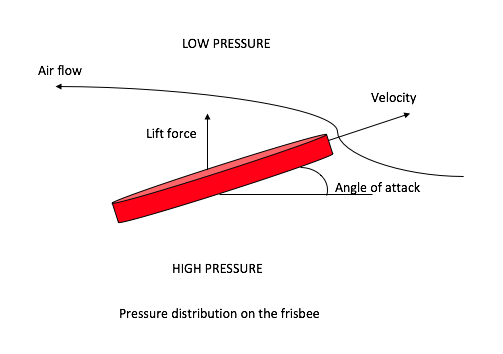
\includegraphics[scale=0.6]{Intro.jpg}
\caption{Pressure distribution on the frisbee}
\label{Pressure distribution on the frisbee}
\end{figure}

\section{Method}
In order to ascertain the optimal throw, we simulated the frisbee's trajectory by computing simulation. This requires to know the velocity and the position of the frisbee at anytime. Since the acceleration modify the velocity through time, we should thus calculate it. This is possible by using the second law of Newton $F = ma$ where $F$ is the force exert on the body of mass $m$ and $a$ is its acceleration. It implies implicitly that we have to find the main forces forces acting on the frisbee,  which are the gravitational force and the lift and drag forces illustrated on the Figure 2. The latter is the force exerts by the air on the frisbee in the flow direction, it is the air resistance. Since these forces only act in the directions parallel and perpendicular to the flow, the simulation can be simplified by only considering those two dimensions.

\begin{figure}[!h]
\centering
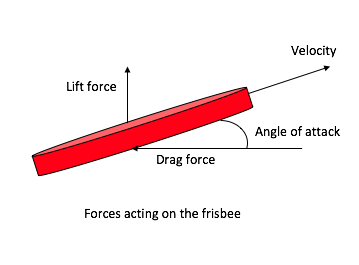
\includegraphics[scale=0.8]{forces.jpg}
\caption{Forces acting on the frisbee}
\label{Forces acting on the frisbee}
\end{figure}

\subsection{Mathematical description}
The three forces cited above are all expressed by physical relationships. In the following part, we will present these relationships.
\\The gravitational force $F_g$ exert on the frisbee is directly proportional to its mass $m$
\[F_g = m g\]
with $g$, the gravitational acceleration.
\\
The drag and lift forces are much difficult to find because the equations depend on the geometry of the object studied, and the object's direction in comparison to the fluid's one. Fortunately, we can approximate the frisbee's geometry to a flat plate moving alongside the flow. In this case, the drag and lift forces are respectively given by :
\[F_d = -\frac{C_d \rho A  v^2}{2}\]
\[F_l = \frac{C_l \rho A  v^2}{2}\]
In this particular case, the fluid is the air, thus $\rho$ is its density, $v$ is the velocity of the Frisbee relative to the air, A is the surface area of the plate exposed to the air flow and $C_d$ and $C_l$ are respectively the drag and lift coefficients.
The drag coefficient, in general, depends on the Reynolds number which gives the type of flow studying. A flow can be laminar or turbulent. The first one relates to ordered flows while the second one caracterise chaotics flows. This number can be calculated with the following relationship:
\[\Re = \frac{\rho v d}{\eta}\]
where the only new term appearing here is $\eta$, the viscosity of the air.
By using the data presented at the result section, we found $Re=2.59$ $10^5$ which correspond to a turbulent flow.
In this case, the drag coefficient can expressed as:
\[C_d = C_{d0} + C_{d\alpha}(\alpha-\alpha_0)^2\]
which links it to the angle of attack $\alpha$. The other terms are constants found experimentally.
\\Finally, the lift coefficient can be found with the relationship below:
\[C_l = C_{l0} + C_{l \alpha} \alpha\]
where $C_{l0}$ and $C_{l\alpha}$ are also constants find by experiments.
\subsection{Numerical modelling}
Solving this problem numerically can be done by using different methods. Here, we will use the Euler progressive method. It simply means that position is calculated from the previous one.
The angle of attack appears in the initial conditions since it represent the angle of the toss. The equations are given below.
\[x = 0 m\]
\[y = 1 m\]
\[v_x = v_i cos(\alpha) \]
\[v_y = v_i sin(\alpha) \] 

where $x$ is the horizontal position, $y$ is the vertical one and $v_x$ and $v_y$ are respectively the horizontal and vertical velocity.
The next positions are calculated by :
\[x_{next} = x_{previous} + v_{x_{previous}} \Delta t \]
\[a_x=\frac{v_{x_{next}}}{\Delta t} = -\frac{C_d \rho A  v_{x_{previous}}^2}{2m}\]
\[y_{next} = y_{previous} + v_{y_{previous}} \Delta t \]
\[a_y = \frac{v_{y_{next}}}{\Delta t} = \frac{C_l \rho A  v_{y_{previous}}^2}{2m} - g\]
where $\Delta t$ is a chosen parameter which represent the time spent between two successive positions
\section{Results}
In this section, we will present three graphs that we obtained from the simulation. All of them were made with the same parameters values except for the angle of attack which is varying from $5\,^{\circ}$ up to $45\,^{\circ} $. 
\\The parameters values are the following:

\begin{tabular}{|l|c|r|}
  \hline
  Symbol & Signification & Value \\
  \hline
  $m$ & Mass of frisbee & 0.175 $kg$\\
  $\rho$ & The density of air & 1.23 $kg/m^3$\\
  $g$ & Acceleration of gravity & 9.81 $m/s^2$ \\
  $d$ & Diameter of Frisbee & 0.26 $m$ \\
  $A$ & Surface area of Frisbee & $\pi (d/2)^2$ $m^2$ \\
  $v_i$ & Initial velocity & 14 $m/s$ \\
  $v_x$ & Initial velocity in the x-direction & $v_icos(\alpha)$ $m/s$ \\
  $v_y$ & Initial velocity in the y-direction & $v_isin(\alpha)$ $m/s$ \\
  $C_{D0}$ & Frisbee dimensional constant & $0.08$ \\
  $C_{L0}$ & Frisbee dimensional constant & $0.15$ \\
  $\alpha_0$ & Frisbee dimensional constant & $-4\pi / 180$ $rad$ \\
  $C_{D\alpha}$ & Frisbee dimensional constant & $2.72$ $rad^{-2}$\\
  $C_{L\alpha}$ & Frisbee dimensional constant & $1.4 $ $rad^{-1}$\\
  
  \hline
\end{tabular}
\begin{figure}[!h]
 \centering
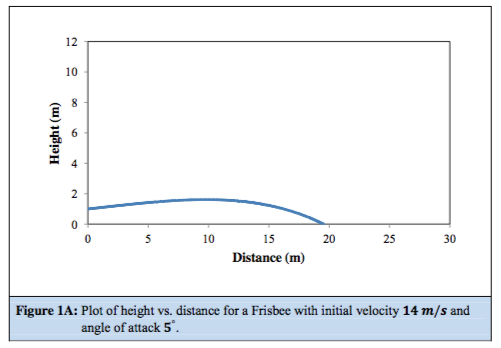
\includegraphics[scale=0.6]{graph1.jpg}
\caption{First result}
\label{First result}
\end{figure}
\\The first graph (figure ~\ref{First result}) shows that an angle of attack of $5\,^{\circ}$ permit to the frisbee to reach a distance of $19m$.
\begin{figure}[!h]
\centering
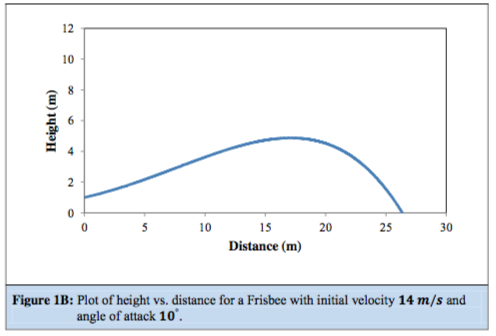
\includegraphics[scale=0.6]{graph2.jpg}
\caption{Second result}
\label{Second result}
\end{figure}
\\The second one (figure ~\ref{Second result}), thrown with an angle of $10\,^{\circ}$ travelled for $26m$.
\begin{figure}[!h]
\centering
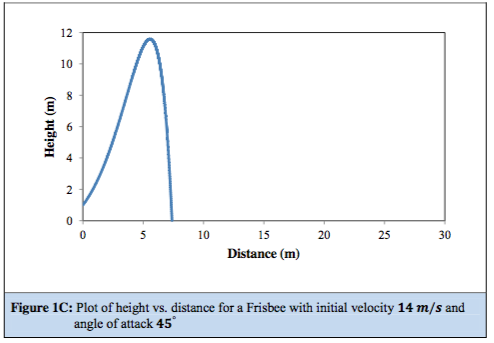
\includegraphics[scale=0.6]{graph3.jpg}
\caption{Third result}
\label{Third result}
\end{figure}
\\The last one (figure ~\ref{Third result}) only glide for $8m$ but was tossed with an angle of $45\,^{\circ} $.

\section{Discussion}
We saw in the different graphs that the angle of attack has an important impact on the distance travelled by the frisbee. The best results were obtain with an angle of $10\,^{\circ}$ which is not an intuitive result. In fact we would rather think that a $45\,^{\circ}$ inclination would allow a higher lift, since this force is the vertical projection of the force applied on the frisbee by the flow. Thus the lower the angle would be(under$45\,^{\circ}$ ), the lower the lift would be. This is the idea shown on Figure 6.
\begin{figure}[!h]
\centering
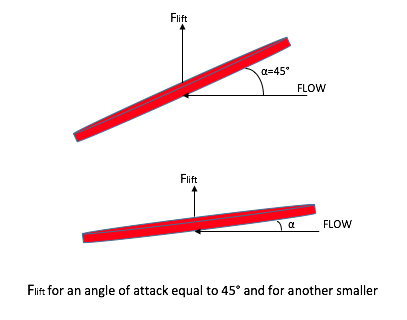
\includegraphics[scale=0.6]{intuitive.jpg}
\caption{Lift cause by the flow for different angle}
\label{Lift cause by the flow for different angle}
\end{figure}
In reality, it is not the case and it is explainable by introducing the concept of recirculation region. When the frisbee's inclination is not null, there is a flow separation. This create two different areas at different pressures. The pressure difference forces the flow to come back in the region where the pressure is lower which is below the frisbee, and is called the recirculation region. This movement of air is opposed to the flow direction, thus it increases the drag force which slow down the frisbee. Therefore the higher is the angle, the higher is drag.
\\Then the optimal angle is nothing else than the result of those two phenomena.
\section{Conclusion}
The basic physics of Frisbee flight turns out to be quite a bit simpler than one might initially expect. It consists of two concepts which are more or less familiar to most people. The first is the gyroscopic stability of rotating objects. It wasn't approached since the purpose of tests were to see how far a standard frisbee can travel. Since the faster a disc rotates,
the more stable its flight; the stability has no direct link to the travel distance. The second is aerodynamic lift. In that case, where there is a lift force, there is a drag force too. The proportion of these too forces needs to be regulated by the angle of attack of the frisbee thrown in order to have the longest distance traveled (which happens to be $10\,^{\circ}$ in this case).

\begin{thebibliography}{9}

\bibitem{art1}
  Hummel, Sarah A.,
  “Frisbee Flight Simulation and Throw Biomechanics”,
  University of Missouri,
  2003.
  
 \bibitem{art2}
  Lissaman P., Hubbard M.,
  “Maximum range of flying discs”,
  University of California,
  2010.
  
  \bibitem{art3}
  Morrison V. R.,
  “The Physics of Frisbees”,
  Mount Allison University,
  2005.

\bibitem{art4}
  Koyanagi R., Seob K., Ohta K., Ohgi Y.,
  “A computer simulation of the flying disc based on the wind tunnel test data”,
  University of Keio \& Yamagata,
  2012.
  
  \bibitem{art5}
  Baumback, Kathleen,
  “The Aerodynamics of Frisbee Flight”,
  University of South Florida,
  2010.
  
  \bibitem{art6}
  Erynn J. Schroeder,
  “An Aerodynamic Simulation of Disc Flight”,
  College of Saint Benedict/Saint John's University,
  2015.

\end{thebibliography}
\end{document}